\input{\string~/Documents/School/"UC Irvine"/ta_template2.0.tex}
\rh{2B}{11.5}
\chead{\today}
\graphicspath{ {\string~/Desktop} }
\usetikzlibrary{arrows}
%============ANSWER KEY TOGGLE===========
\newcommand{\ans}[1]{ \noindent {\color{red} \textbf{Answer:} #1}}
%\renewcommand{\ans}[1]{\vspace{3in}}
%==========================================
\begin{document}
\begin{center}
\textbf{Alternating Series Test}
\end{center}

\begin{thm}[Alternating Series Test]
\label{thm:ast}
If the alternating series:
\[
\sum_{n = 1}^\infty \lrp{-1}^{n-1} b_n = b_1 - b_2 + b_3 - \cdots \mte{ with } b_n > 0
\]
satisfies the following conditions:
\begin{enumerate}[label= $\roman*.$]
\item $b_{n+1} \leq b_n$ for all $n$ and
\item $\lim_{n \to \infty} b_n = 0$
\end{enumerate}
Then the series converges. 
\[
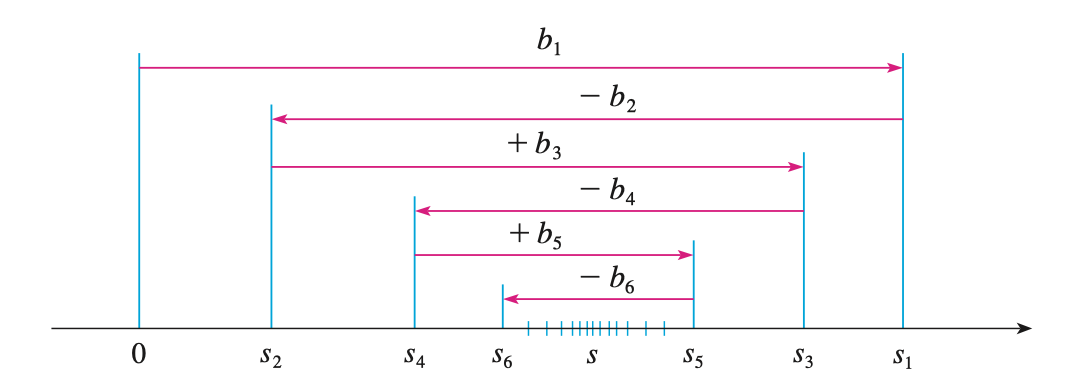
\includegraphics[width=0.7\textwidth]{fig1.png}
\]
\end{thm}

\begin{thm}[Alternating Series Estimation Theorem]
If we have the alternating series $S = \sum (-1)^{n-1} b_n$ where $b_n >0$ satisfying $(i)$ and $(ii)$, then 
\[
\lrabs{R_n} = \lrabs{s - s_n} \leq b_{n+1}
\]
\end{thm}
\begin{aun}
From the picture, we see that the terms in absolute value get close to the limit. 
\end{aun}

\begin{exx}
Consider the alternating harmonic series:
\[
\sum_{n = 1}^\infty \frac{(-1)^n}{n}
\]
Determine whether this series diverges, and if so, determine the remainder at the $n = 5$ term. 
\end{exx}
\ans{We'll show that this series satisfies the conditions from Theorem~\ref{thm:ast}:
\begin{enumerate}[label=(\roman*)]
\item We know that:
\[
\frac{1}{n+1} < \frac{1}{n} \checkmark
\]
\item We also have that:
\[
\lim_{n \to \infty} \frac1n = 0 \checkmark
\]
\end{enumerate}
Thus, by Theorem~\ref{thm:ast}, we have convergence. To estimate at the $5$th term, we see:
\[
\lrabs{s - s_5} \leq \frac{1}{5 + 1} \mte{ and thus } -\frac16 \leq s - s_5 \leq \frac16
\]
Substituting for what we know, we have:
\[
s_5 = \sum_{n = 1}^5 \frac1n = \frac{-47}{60} 
\]
This gives:
\[
-\frac16 \leq s + \frac{47}{60}  \leq \frac16 \mte{ so } -\frac16 - \frac{47}{60} \leq s   \leq \frac16 - \frac{47}{60}
\]
}

\problembox{Determine if the following series converges or diverges:
\[\sum_{n=1}^{\infty} \frac{(-1)^{n-1}}{7+2 n}\]
}
\ans{The sequence $\frac{1}{7 + 2n}$ is decreasing and has limit = 0, so converges by Theorem~\ref{thm:ast}}

\problembox{Determine if the following series converges or diverges:
\[
\sum_{n = 1}^\infty \frac{(-1)^{n-1} n^2}{n^3 + 4}
\]
}
\ans{Converges by the same reason as the earlier problem.}

\end{document}